\documentclass[english]{SPFShortReport}
\usepackage{subfigure}
\usepackage{spfFigures}
\usepackage{longtable}
\usepackage{url}
\usepackage{gensymb}
\usepackage[yyyymmdd,hhmmss]{datetime}
\reportName{Python calculation for heat pump SIN-26TU}
\reportSubName{Parametric Heat Pump calculation} 
\reportDate{\today \hspace{0.1cm} at: \currenttime \hspace{0.1cm} h} 
\author{Dani Carbonell}
\address{dani.carbonell@solarenergy.ch}
\begin{document}
\begin{table}[!ht]
\begin{small}
\caption{Fitted coefficients for the heat pump.}
\begin{center}
\resizebox{12cm}{!} 
{
\begin{tabular}{l | c c } 
\hline
\hline
Coefficient &Description & \\ 
 & &$[kW]$\\ 
\hline
$PQ_{1}$ & \emph{$1^{st}$ condenser polynomial coefficient}  & 2.5644e+01    \\ 
$PQ_{2}$ & \emph{$2^{st}$ condenser polynomial coefficient}  & 3.0014e+02    \\ 
$PQ_{3}$ & \emph{$3^{st}$ condenser polynomial coefficient}  & 5.9163e+01    \\ 
$PQ_{4}$ & \emph{$4^{st}$ condenser polynomial coefficient}  & -5.9720e+02    \\ 
$PQ_{5}$ & \emph{$5^{st}$ condenser polynomial coefficient}  & 5.1391e+02    \\ 
$PQ_{6}$ & \emph{$6^{st}$ condenser polynomial coefficient}  & -2.9866e+02    \\ 
\hline
$PCOP_{1}$ & \emph{$1^{st}$ COP polynomial coefficient}  & 6.7660e+00    \\ 
$PCOP_{2}$ & \emph{$2^{st}$ COP polynomial coefficient}  & 7.0047e+01    \\ 
$PCOP_{3}$ & \emph{$3^{st}$ COP polynomial coefficient}  & -5.1288e+00    \\ 
$PCOP_{4}$ & \emph{$4^{st}$ COP polynomial coefficient}  & -2.9395e+02    \\ 
$PCOP_{5}$ & \emph{$5^{st}$ COP polynomial coefficient}  & 1.0724e+02    \\ 
$PCOP_{6}$ & \emph{$6^{st}$ COP polynomial coefficient}  & -7.2713e+01    \\ 
\hline
$\dot m_{cond}$ & 4500.00 $[kg/h]$\\ 
$\dot m_{evap}$ & 4500.00 $[kg/h]$\\ 
\hline
$COP_{nom}$ (B0W35)& 4.85 \\ 
$Q_{c,nom}$ (B0W35)& 26.63 kW\\ 
$COP_{nom}$ (B2W35)& 5.09 \\ 
$Q_{c,nom}$ (B2W35)& 28.15 kW\\ 
$COP_{nom}$ (B10W35)& 6.18 \\ 
$Q_{c,nom}$ (B10W35)& 34.70 kW\\ 
\hline
\hline
\end{tabular}
}
\label{CoefTable}
\end{center}
\end{small}
\end{table}
\begin{table}[!ht]
\begin{small}
\caption{Predicting results of the heat pump.}
\begin{center}
\resizebox{12cm}{!} 
{
\begin{tabular}{l | c c c c c c c c c c c } 
\hline
\hline
$T_{evap,in}$ &$T_{evap,out}$ &$T_{cond,in}$ &$T_{cond,out}$ &$COP$ &$Q_{cond}$ &$Q_{evap}$ &$W_{comp}$ &$\dot m_{cond}$ &$\dot m_{evap}$ &$\Delta T_{evap}$ &$\Delta T_{cond}$ \\ 
$^oC$ &$^oC$ &$^oC$ &$^oC$ &$[-]$ &$[kW]$ &$[kW]$ &$[kW]$ &kg/h &kg/h &K &K\\ 
\hline
-7.00 & -10.46 & 25.90 & 30.00 & 4.31 & 21.46 & 16.48 & 4.98 & 4500 & 4500 & 3.5 & 4.1\\ 
-7.00 & -10.39 & 34.60 & 38.75 & 3.90 & 21.72 & 16.16 & 5.57 & 4500 & 4500 & 3.4 & 4.1\\ 
-7.00 & -10.15 & 43.41 & 47.50 & 3.34 & 21.42 & 15.01 & 6.41 & 4500 & 4500 & 3.1 & 4.1\\ 
-7.00 & -9.66 & 52.33 & 56.25 & 2.62 & 20.55 & 12.70 & 7.84 & 4500 & 4500 & 2.7 & 3.9\\ 
-7.00 & -8.68 & 61.35 & 65.00 & 1.72 & 19.12 & 8.00 & 11.12 & 4500 & 4500 & 1.7 & 3.7\\ 
-4.00 & -7.89 & 25.49 & 30.00 & 4.67 & 23.60 & 18.55 & 5.05 & 4500 & 4500 & 3.9 & 4.5\\ 
-4.00 & -7.78 & 34.22 & 38.75 & 4.17 & 23.71 & 18.02 & 5.69 & 4500 & 4500 & 3.8 & 4.5\\ 
-4.00 & -7.49 & 43.06 & 47.50 & 3.52 & 23.24 & 16.63 & 6.61 & 4500 & 4500 & 3.5 & 4.4\\ 
-4.00 & -6.93 & 52.01 & 56.25 & 2.70 & 22.21 & 13.99 & 8.22 & 4500 & 4500 & 2.9 & 4.2\\ 
-4.00 & -5.79 & 61.06 & 65.00 & 1.71 & 20.65 & 8.54 & 12.11 & 4500 & 4500 & 1.8 & 3.9\\ 
-1.00 & -5.35 & 25.06 & 30.00 & 5.06 & 25.85 & 20.74 & 5.11 & 4500 & 4500 & 4.3 & 4.9\\ 
-1.00 & -5.20 & 33.83 & 38.75 & 4.46 & 25.79 & 20.02 & 5.78 & 4500 & 4500 & 4.2 & 4.9\\ 
-1.00 & -4.86 & 42.69 & 47.50 & 3.72 & 25.17 & 18.40 & 6.77 & 4500 & 4500 & 3.9 & 4.8\\ 
-1.00 & -4.24 & 51.67 & 56.25 & 2.81 & 23.98 & 15.44 & 8.53 & 4500 & 4500 & 3.2 & 4.6\\ 
-1.00 & -2.96 & 60.74 & 65.00 & 1.72 & 22.29 & 9.34 & 12.95 & 4500 & 4500 & 2.0 & 4.3\\ 
2.00 & -2.83 & 24.61 & 30.00 & 5.46 & 28.21 & 23.05 & 5.16 & 4500 & 4500 & 4.8 & 5.4\\ 
2.00 & -2.64 & 33.41 & 38.75 & 4.78 & 27.99 & 22.14 & 5.85 & 4500 & 4500 & 4.6 & 5.3\\ 
2.00 & -2.26 & 42.31 & 47.50 & 3.95 & 27.20 & 20.31 & 6.89 & 4500 & 4500 & 4.3 & 5.2\\ 
2.00 & -1.58 & 51.31 & 56.25 & 2.95 & 25.85 & 17.08 & 8.77 & 4500 & 4500 & 3.6 & 4.9\\ 
2.00 & -0.19 & 60.41 & 65.00 & 1.77 & 24.03 & 10.43 & 13.61 & 4500 & 4500 & 2.2 & 4.6\\ 
5.00 & -0.34 & 24.14 & 30.00 & 5.90 & 30.67 & 25.47 & 5.20 & 4500 & 4500 & 5.3 & 5.9\\ 
5.00 & -0.11 & 32.97 & 38.75 & 5.13 & 30.29 & 24.38 & 5.90 & 4500 & 4500 & 5.1 & 5.8\\ 
5.00 & 0.31 & 41.90 & 47.50 & 4.20 & 29.34 & 22.36 & 6.98 & 4500 & 4500 & 4.7 & 5.6\\ 
5.00 & 1.04 & 50.93 & 56.25 & 3.11 & 27.84 & 18.89 & 8.95 & 4500 & 4500 & 4.0 & 5.3\\ 
5.00 & 2.52 & 60.06 & 65.00 & 1.84 & 25.88 & 11.82 & 14.07 & 4500 & 4500 & 2.5 & 4.9\\ 
8.00 & 2.13 & 23.66 & 30.00 & 6.36 & 33.23 & 28.00 & 5.22 & 4500 & 4500 & 5.9 & 6.3\\ 
8.00 & 2.39 & 32.51 & 38.75 & 5.50 & 32.69 & 26.75 & 5.94 & 4500 & 4500 & 5.6 & 6.2\\ 
8.00 & 2.85 & 41.47 & 47.50 & 4.49 & 31.59 & 24.55 & 7.04 & 4500 & 4500 & 5.1 & 6.0\\ 
8.00 & 3.63 & 50.53 & 56.25 & 3.30 & 29.93 & 20.87 & 9.07 & 4500 & 4500 & 4.4 & 5.7\\ 
8.00 & 5.17 & 59.68 & 65.00 & 1.94 & 27.84 & 13.50 & 14.34 & 4500 & 4500 & 2.8 & 5.3\\ 
11.00 & 4.57 & 23.15 & 30.00 & 6.85 & 35.89 & 30.65 & 5.24 & 4500 & 4500 & 6.4 & 6.9\\ 
11.00 & 4.87 & 32.03 & 38.75 & 5.90 & 35.20 & 29.23 & 5.97 & 4500 & 4500 & 6.1 & 6.7\\ 
11.00 & 5.37 & 41.02 & 47.50 & 4.79 & 33.94 & 26.86 & 7.08 & 4500 & 4500 & 5.6 & 6.5\\ 
11.00 & 6.18 & 50.12 & 56.25 & 3.52 & 32.13 & 23.00 & 9.13 & 4500 & 4500 & 4.8 & 6.1\\ 
11.00 & 7.76 & 59.29 & 65.00 & 2.07 & 29.89 & 15.45 & 14.44 & 4500 & 4500 & 3.2 & 5.7\\ 
14.00 & 7.00 & 22.62 & 30.00 & 7.36 & 38.66 & 33.40 & 5.25 & 4500 & 4500 & 7.0 & 7.4\\ 
14.00 & 7.33 & 31.53 & 38.75 & 6.32 & 37.81 & 31.83 & 5.98 & 4500 & 4500 & 6.7 & 7.2\\ 
14.00 & 7.86 & 40.55 & 47.50 & 5.13 & 36.40 & 29.30 & 7.10 & 4500 & 4500 & 6.1 & 7.0\\ 
14.00 & 8.70 & 49.68 & 56.25 & 3.77 & 34.43 & 25.29 & 9.15 & 4500 & 4500 & 5.3 & 6.6\\ 
14.00 & 10.30 & 58.88 & 65.00 & 2.23 & 32.05 & 17.65 & 14.39 & 4500 & 4500 & 3.7 & 6.1\\ 
17.00 & 9.40 & 22.07 & 30.00 & 7.90 & 41.52 & 36.26 & 5.26 & 4500 & 4500 & 7.6 & 7.9\\ 
17.00 & 9.76 & 31.01 & 38.75 & 6.77 & 40.53 & 34.55 & 5.98 & 4500 & 4500 & 7.2 & 7.7\\ 
17.00 & 10.32 & 40.06 & 47.50 & 5.49 & 38.96 & 31.87 & 7.10 & 4500 & 4500 & 6.7 & 7.4\\ 
17.00 & 11.19 & 49.22 & 56.25 & 4.04 & 36.84 & 27.72 & 9.12 & 4500 & 4500 & 5.8 & 7.0\\ 
17.00 & 12.79 & 58.45 & 65.00 & 2.41 & 34.30 & 20.07 & 14.23 & 4500 & 4500 & 4.2 & 6.5\\ 
20.00 & 11.78 & 21.51 & 30.00 & 8.46 & 44.49 & 39.23 & 5.26 & 4500 & 4500 & 8.2 & 8.5\\ 
20.00 & 12.17 & 30.47 & 38.75 & 7.25 & 43.34 & 37.37 & 5.98 & 4500 & 4500 & 7.8 & 8.3\\ 
20.00 & 12.76 & 39.55 & 47.50 & 5.88 & 41.63 & 34.55 & 7.08 & 4500 & 4500 & 7.2 & 7.9\\ 
20.00 & 13.65 & 48.74 & 56.25 & 4.34 & 39.35 & 30.28 & 9.07 & 4500 & 4500 & 6.3 & 7.5\\ 
20.00 & 15.25 & 58.00 & 65.00 & 2.62 & 36.65 & 22.67 & 13.99 & 4500 & 4500 & 4.8 & 7.0\\ 
\hline
\hline
\end{tabular}
}
\label{ResultsTable}
\end{center}
\end{small}
\end{table}
\begin{figure}[!ht]
\begin{center}
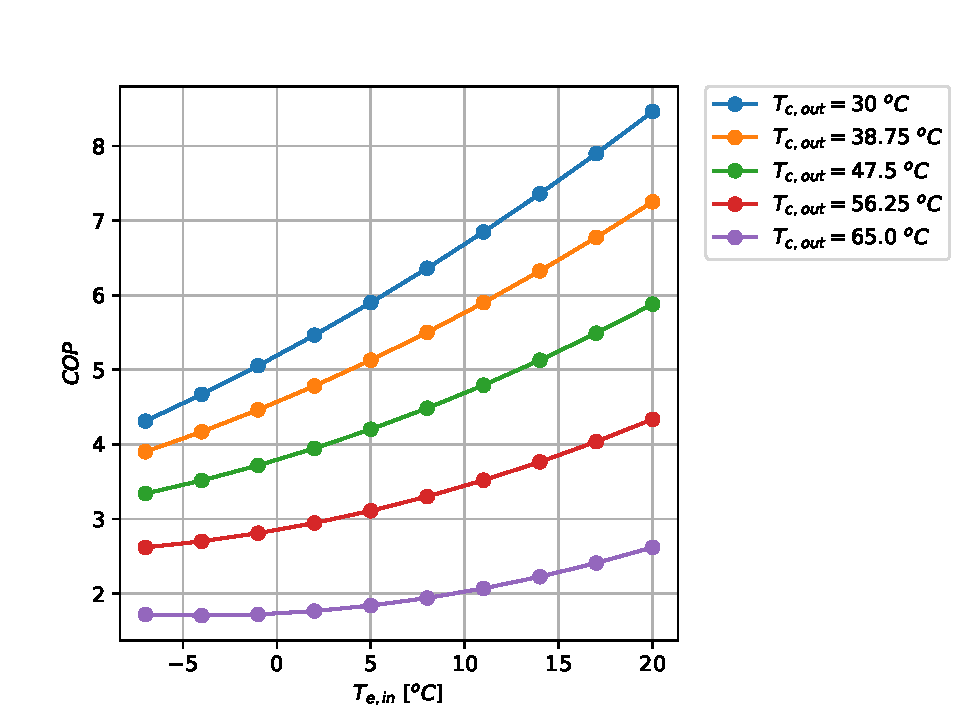
\includegraphics[width=1\textwidth]{C:/Daten/spfPackages/GIT/spfTrnsysFiles/HeatPump/BrineToWater/Walter Meier/SIN-26TU/SIN-26TU-Cop.pdf}
\caption{COP Results for the heat pump at the selected points}
\label{COPFig}
\end{center}
\end{figure}
\begin{figure}[!ht]
\begin{center}
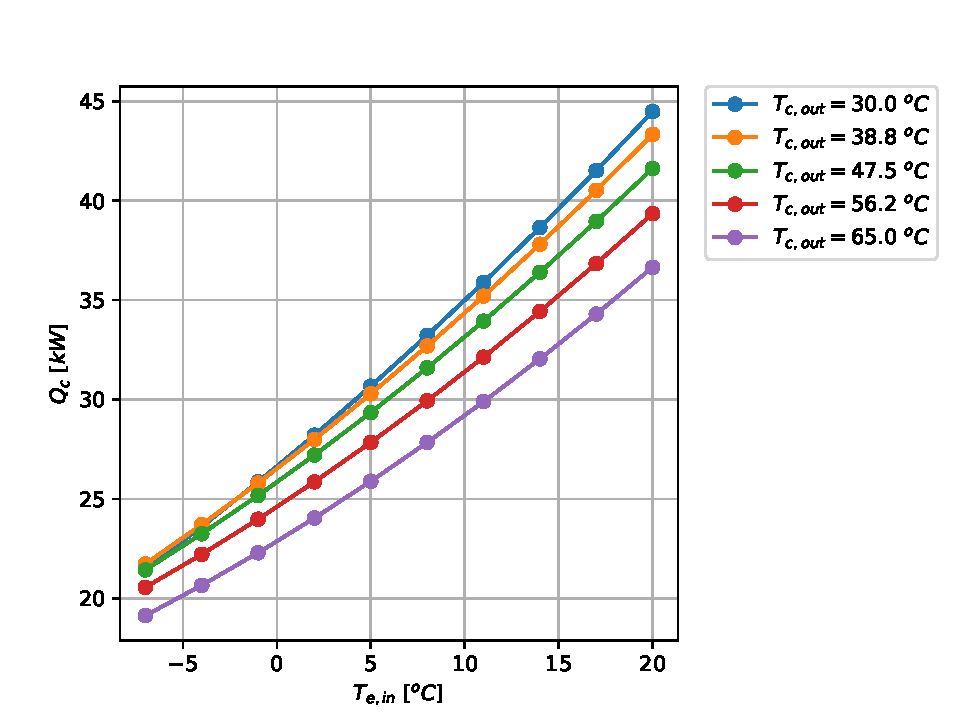
\includegraphics[width=1\textwidth]{C:/Daten/spfPackages/GIT/spfTrnsysFiles/HeatPump/BrineToWater/Walter Meier/SIN-26TU/SIN-26TU-Qc.pdf}
\caption{$Q_c$ Results for the heat pump at the selected points}
\label{QcFig}
\end{center}
\end{figure}
\end{document}
